\section{Background: Casual Tracing} \label{sec:background}

\begin{figure}[tb]
	\footnotesize
    \centering
	 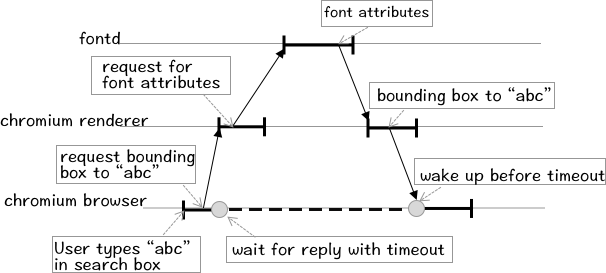
\includegraphics[width=\columnwidth]{./figures/causaltracing_example.png}
    \caption{Handling User Typing in Chromium.  The \vv{browser} and
      \vv{render} each split the work among a main thread and a worker
      thread.  Front service daemon \vv{fontd} uses thread pooling.  For
      clarity, only processes are shown, not their threads.}
    \label{fig:chromium-normal}
\end{figure}

Modern applications are often highly concurrent, spreading the handling of
an external request in multiple threads, processes, and asynchronous
contexts, each of which may multiplex on different requests.  Causal
tracing thus aims to reconnect the execution segments physically separated
in different execution contexts but logically on behalf of the same
request.  Figure~\ref{fig:chromium-normal} shows an example in Chromium,
an open-source browser engine that powers Google Chrome and, starting
recently, Microsoft Edge~\cite{chromiumurl}. When a user types a string in
Chromium, the \vv{browser} process sends an IPC message to the \vv{render}
process where the rendering view and WebKit code run, to calculate the
bounding box of the string.  \vv{render} then queries \vv{fontd}, the font
service daemon, for font dimensions.  Once \vv{fontd} replies and wakes up
\vv{render}, \vv{render} in turn wakes up \vv{browser}.  The handling of user
typing is thus split among at least three processes and their relevant
threads, and an ideal causal tracing tool would capture these segments
(vertices) and their connections (edges) into a generalized control-flow
graph to aid developer reasoning.

Compared to tools such as \spindump that capture only the current system
state such as the call stack snapshots of each thread, causal tracing
captures the dependency path of events, enabling users to trace across
threads and processes to past events.  For instance, if \vv{render}'s
reply hangs \vv{browser}, causal tracing would enable a developer to
examine \vv{fontd}'s reply to \vv{render}, whereas the \vv{fontd} call
stack that \spindump captures at the time of the hang may be for a
completely irrelevant request.

Mechanically, to build an event graph, causal tracing tools must infer the
beginning and ending boundaries of execution segments and connect a
segment with the other segments that it creates or wakes up. Lacking
application semantics, existing tools make various assumptions to infer
segment boundaries and connections.  We select AppInsight and Panappticon,
two tools closely related to \xxx, and describe how they do so.

AppInsight is designed to help developers understand the performance
bottlenecks in mobile applications.  To infer execution segment
boundaries, it interposes on the interface between the application and
framework, and assumes that the application follows mostly the event
callback programming idiom.  The entry and exit of a callback invocation
delimit an execution segment.  If this segment installs additional
callbacks or signals a waiting thread, then AppInsight connects the
corresponding segments.

Panappticon detects performance issues in Android applications. It traces
low-level events in the Android system and libraries.  To infer execution
segment boundaries and connections, it assumes two programming idioms:
work queue and thread pooling.  For work queue, it marks the handling of a
work item as an execution segment, and connects this segment to the
segment that dispatches the work item.  For thread pooling, it marks from
the wakeup of a worker thread to the wait as an execution segment, and
connects this segment to the segment waking up the worker thread.

%% In this section, we illustrate causal tracing and prior work on it. Causal
%% tracing collects events standing for instrucions executed in CPU and generates
%% a graphical representation with traced events as vertices. Two events always
%% following a sequential constraint reflects causality, which is represented
%% as an edge. The graph helps users understand the complex causal behaviors across
%% thread/process boundaries and attribute bugs to their root causes. Prior works
%% have different definitions of vertices, edges, and root causes based on what
%% events are collected.

%% AppInsight instruments all the upcalls from the framework to the application.
%% It traces user input, display update, the begin and end of procedual call, the
%% invocation of callback function, exception and blocking events in threads. Each
%% event is reflected as a vertex in the request graph. Therefore, the request
%% graph connects (1)user input event to (2)the beginning of event handler, which
%% in turn connects to (3)the beginning of callback in background threads. The
%% vertices like (2) and (3) will connect to (4)the end of the procedual call
%% or lead to (5 )exception. Besides, they will also connect to (6)blocking for
%% signal, if the execution requires synchronization. The goal of AppInsight is to
%% help developers understand the performance bottlenecks with critical paths or
%% exception paths. It defines the root cause as the state of a function execution,
%% long blocking or exception in the application.

%% To be unobtrusive, Panappticon instruments the system to collect low-level
%% and fine grained events from libraries and kernel, including user input,
%% display update, asynchronous call and callback, inter-process comminication,
%% synchronization mechanism, and resource accounting. Every event is a vertex.
%% Panappticon connects continuous vertices which stem from atomic work in a
%% thread, \eg, a worker thread processing one task from a task queue, into an
%% execution interval. Two execution intervals are connected if the earlier
%% interval triggers the latter one. For example, a user input triggering an
%% enqueue message in the same thread reflects as an execution interval, where
%% two vertices are connected with a temperal ordering edge. In another thread,
%% dequeuing the message and submiting an asynchronous task generate another
%% execution interval. The two intervals are connected with a causal edge. With the
%% resouces analysis in every user transaction, from user input to display update,
%% Panapption speculates and manually inspect root causes from design flaws, harmful
%% interaction, to underpowered hardware.
